\chapter{THIẾT KẾ VÀ TÍCH HỢP AI}
\label{ch:08}

\section{Kiến trúc Pipeline AI 2 lớp (Dual-layer Resilience)}
Hệ thống tích hợp Pipeline AI 2 lớp linh hoạt (Hình~\ref{fig:ai_pipe}):
\begin{figure}[htbp]
    \centering
    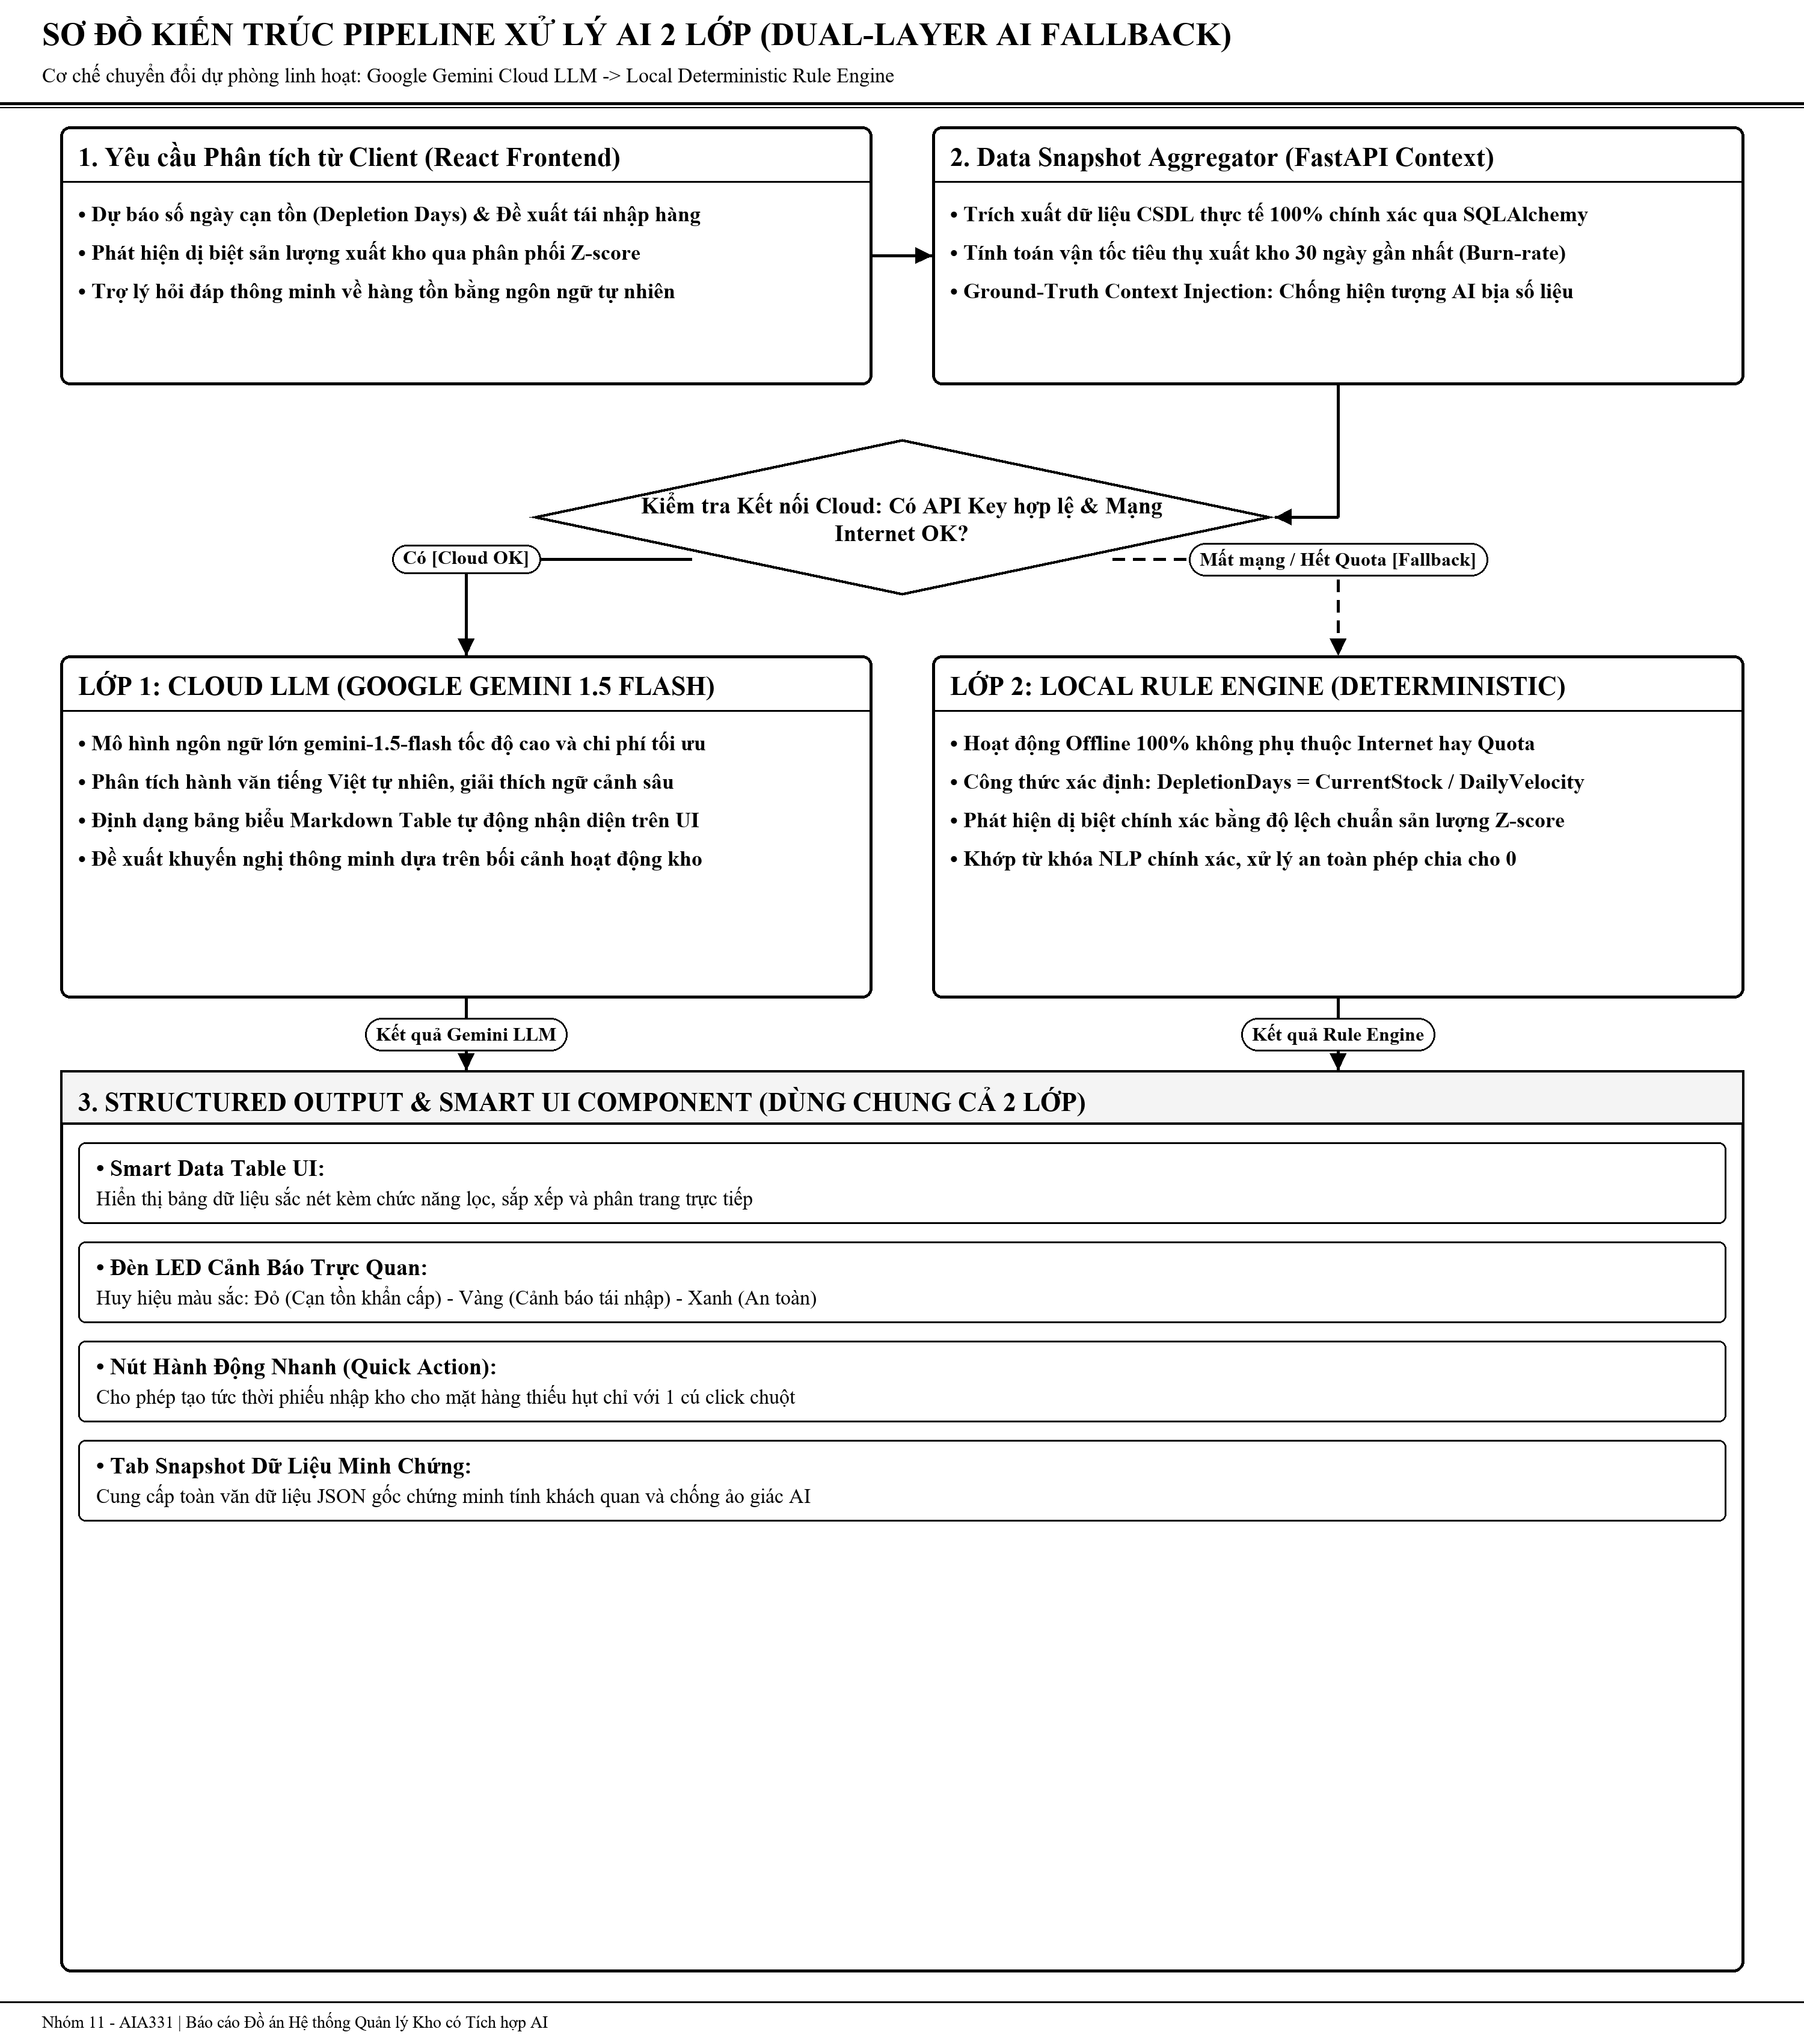
\includegraphics[width=0.92\textwidth]{07_so_do_pipeline_ai_fallback.png}
    \caption{Sơ đồ kiến trúc Pipeline AI 2 lớp linh hoạt (Nhóm 11)}
    \label{fig:ai_pipe}
\end{figure}

\section{Trợ lý Hỏi Đáp Kho AI Tự Nhiên (NLP Assistant)}
Hình~\ref{fig:seq_ai} thể hiện sơ đồ tuần tự xử lý câu hỏi tự nhiên của thủ kho và phản hồi trực quan.
\begin{figure}[htbp]
    \centering
    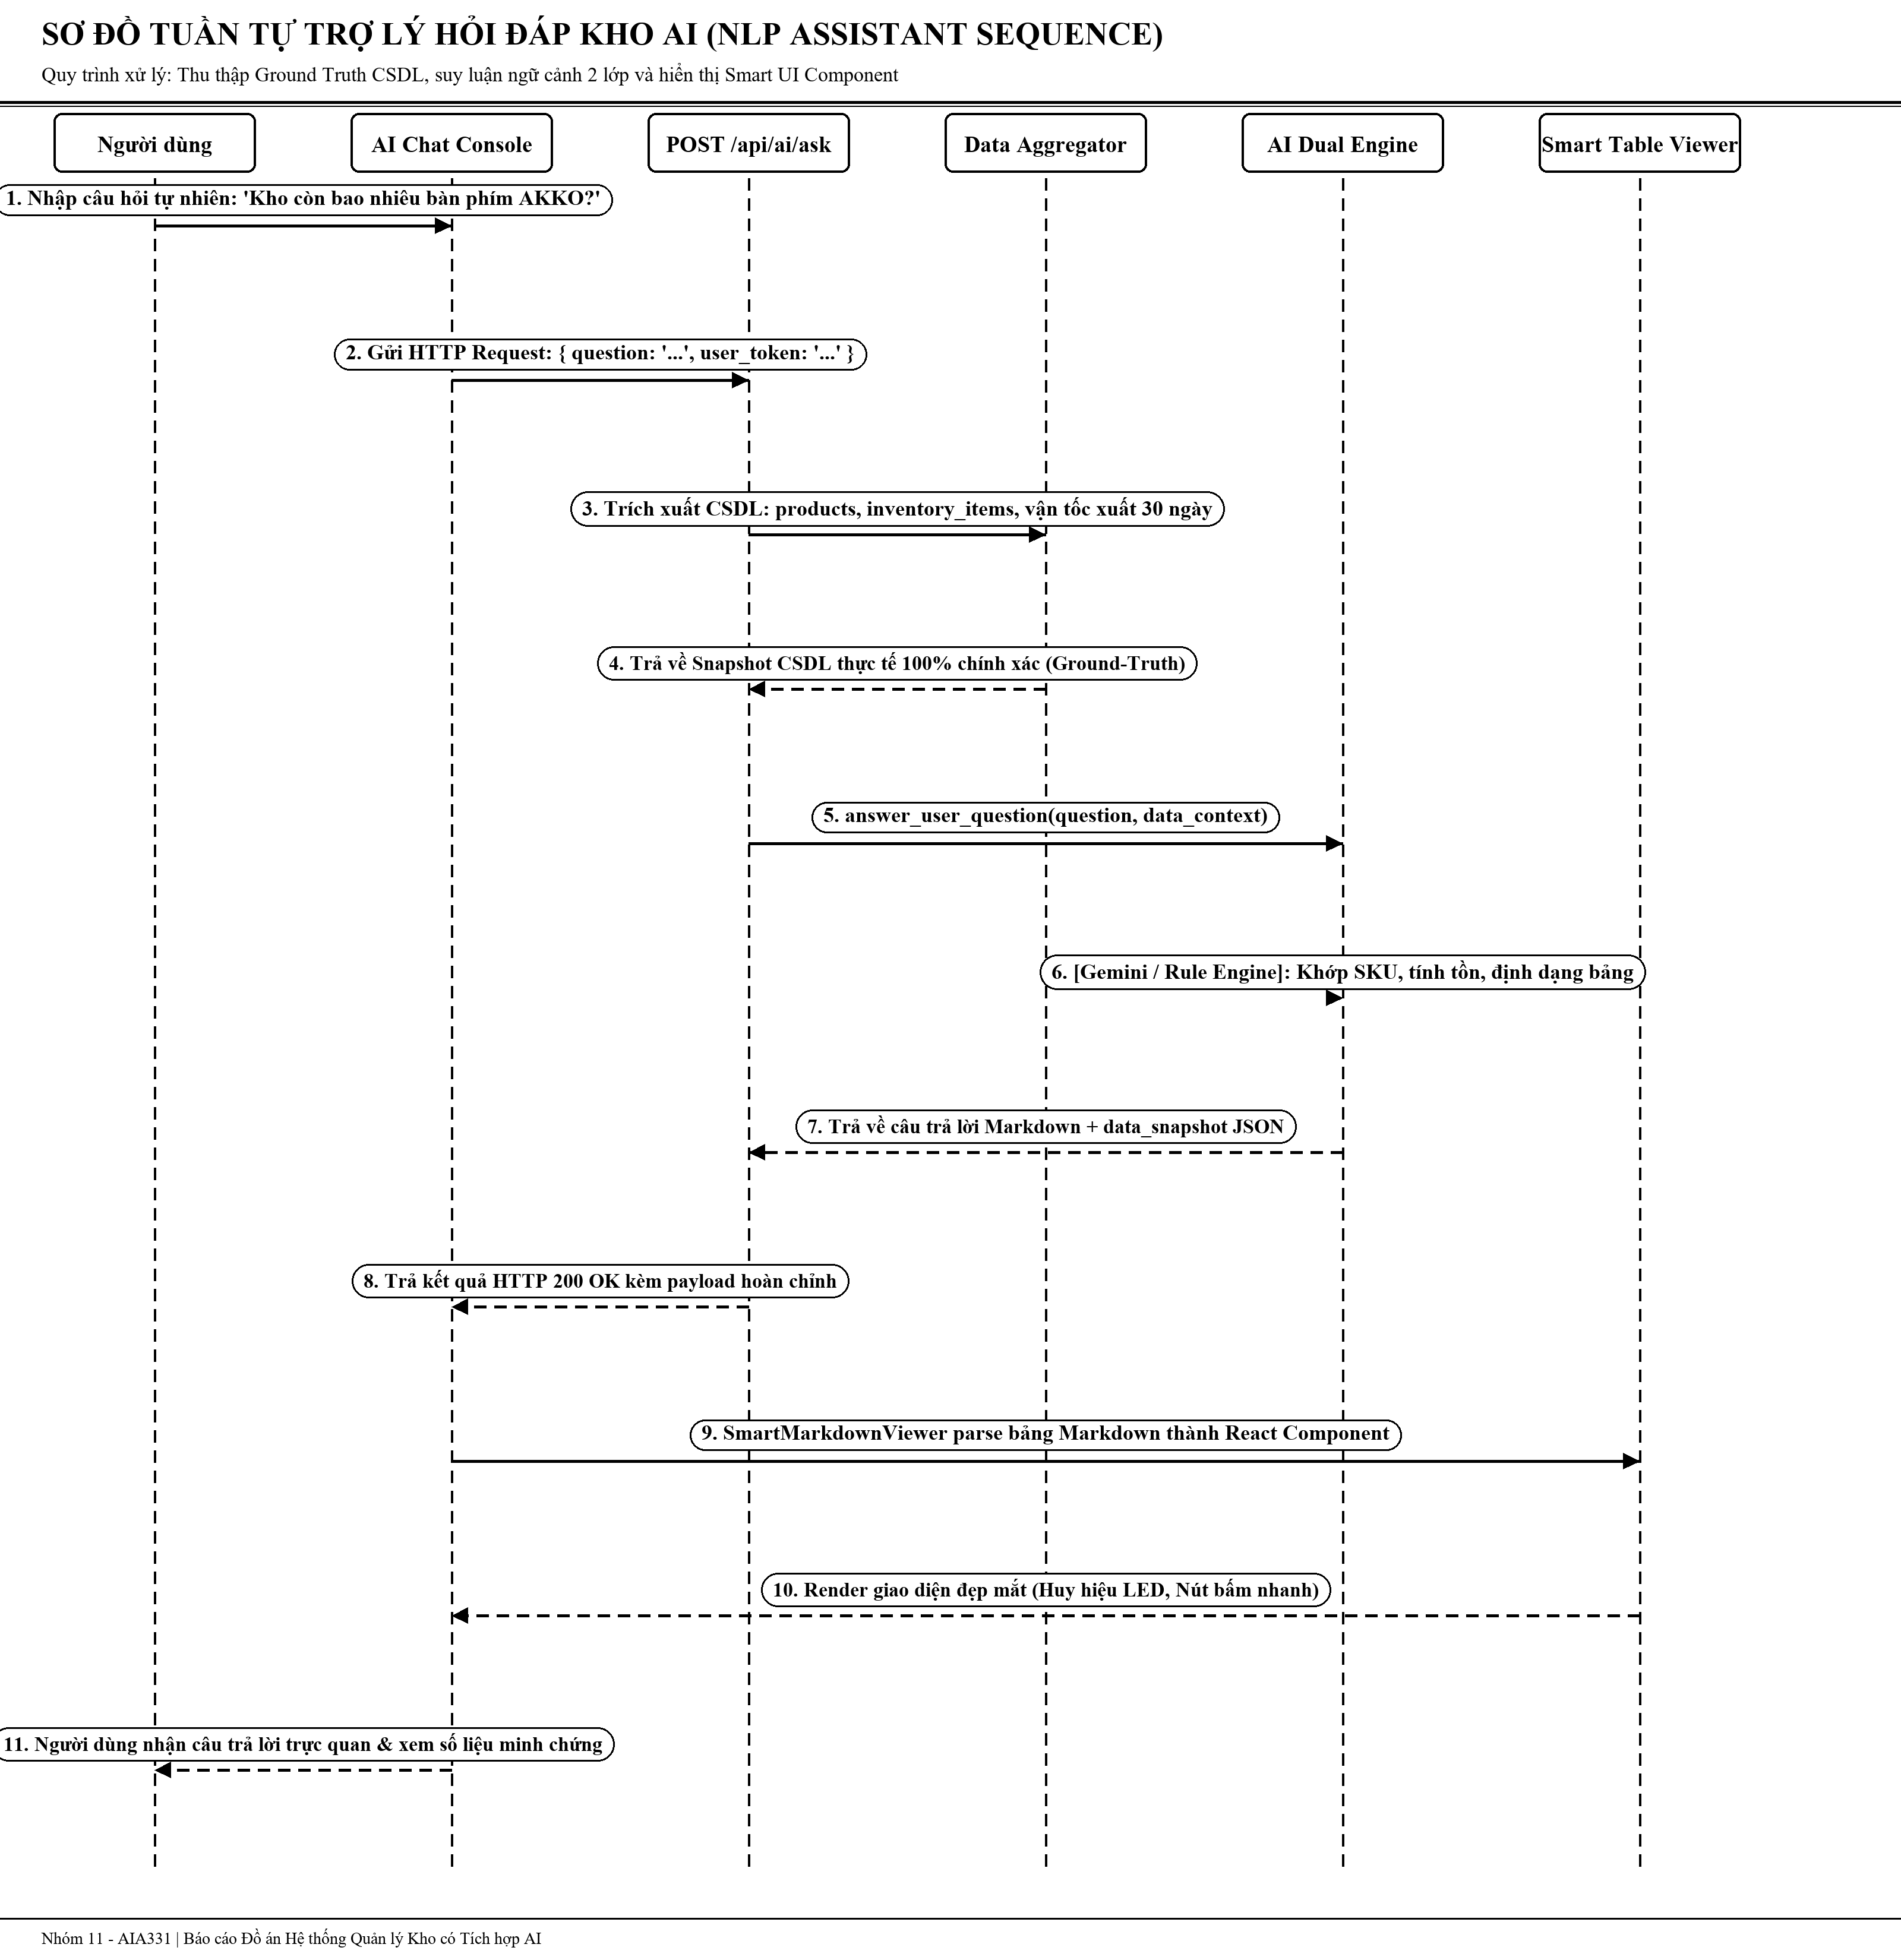
\includegraphics[width=0.90\textwidth]{08_so_do_tuan_tu_hoi_dap_ai.png}
    \caption{Sơ đồ tuần tự Trợ lý hỏi đáp kho bằng ngôn ngữ tự nhiên}
    \label{fig:seq_ai}
\end{figure}
